\documentclass[10pt]{article}
%\usepackage[margin=1in]{geometry}
\usepackage{amsmath,amssymb,graphicx}
\usepackage{hyperref}
\usepackage{mathtools}
\setlength\parindent{0pt}
\begin{document}
\title{Assignment 2: Advection Diffusion Reaction equation}
\author{1212550}
\begin{center}
\section*{Assignment 2: Advection Diffusion Reaction equation}


The following is a brief report concerning the implementation\\ of my class $\textit{Finite.cc}$ upon specific test cases.\\
\end{center}

\section{Finite Difference method}

\subsection{Introducing the problem}

The following is the (1-D) linear advection diffusion reaction equation. Given $f \in C([0,L])$, we want to find $u \in C^2(0,L)$ such that
\[ -\alpha u'' + \beta u' + \gamma u = f,~\text{in}~(0,L), \quad (\star)\]
with respect to certain boundary conditions, (where $\alpha,\beta,\gamma \in \mathbb{R}$ constant). In this report we will considering a discretisation of the above equation based on the $\textit{finite difference}$ (FD) approach. In particular, we will be looking at the advection diffusion problem
\[ -\alpha u'' + \beta u' = 0,~\quad u(0)=0,~u(L)=1, \quad(\dagger) \]
where, without loss of generality, we suppose $L=1$. Let the spatial operator $\mathcal{L}$ be defined such that $\mathcal{L}[u] =  -\alpha u'' + \beta u'$. We will be evaluating $\mathcal{L}$ at a set of points $\{ x_j \}_{j=0}^{J+1}$, which partitions the interval $[0,1]$. We will use a uniform mesh size $h$, such that $h \coloneqq |(x_{j-1},x_j)| = \frac{1}{J+1}$.

In the FD approach, derivatives are replaced with difference quotients of the approximate solution $U$, obtained by truncating the Taylor expansion of the exact solution $u$ around the point $x_j$. These approximations can the be stated succinctly using the following difference operators,
\begin{align*}
    \partial^+U_j &\coloneqq \frac{U_{j+1} - U_j}{h}, \quad \text{(Forward difference)} \\
    \partial^-U_j &\coloneqq \frac{U_j - U_{j-1}}{h}, \quad \text{(Backward difference)} \\
    \partial^0 &\coloneqq \frac{1}{2}(\partial^+ + \partial^-). \quad \text{(Central difference)}
\end{align*}
In particular, a discrete problem approximating $(\dagger)$ is, for $j=1,...,J$, find $U_j$ such that
\begin{align*}
&\mathcal{L}_h[U_j] \coloneqq[-\alpha \partial^-\partial^+ + \beta \partial^0]U_j = 0, \\
&U_0 = 0,~U_1 = 1.
\end{align*}
To solve this discrete problem we can first describe the operator in matrix format, denoted by $A \in \mathbb{R}^{J\times J}$, such that $AU=f$. By calculating the coefficients for $U_{j-1},U_j$ and $U_{j+1}$ from the above equation, we see that the upper-diagonal, diagonal and lower-diagonal values of the matrix must be
\[ -\frac{\alpha}{h^2} + \frac{\beta}{2h}, \quad
\frac{2 \alpha}{h^2}, \quad
-\frac{\alpha}{h^2} - \frac{\beta}{2h}, \]
respectively. All other entries must be zero. Furthermore, due to the boundary conditions required by $(\dagger)$, we must have
\[ f = \Big(0,...,0,\frac{\alpha}{h^2} - \frac{\beta}{2h}\Big)^T \in \mathbb{R}^{J \times 1}.\]
Depending on the values of $\alpha$ and $\beta$, the problem is now potentially solvable via matrix inversion. In particular to this assignment, we aim to do this via the $\textit{Gauss Seidel}$ algorithm.

Note that for equation $(\dagger)$, we can compute its true (analytic) solution via ordinary differential equation methods. Indeed, the solution to this problem is
\[ u(x) = \frac{1}{e^{\frac{\beta}{\alpha}} - 1}(e^{\frac{\beta}{\alpha}x} -1). \]
Ideally, we would like to be in the case where the approximate solution converges to the analytic solution at the grid points, as the mesh size $h$ gets smaller. Assuming the analytic and discrete problem have unique solutions, this will happen if the method is consistent and stable. This result is know as the $\textit{Fundamental Theorem of Numerical Analysis for FD methods}$.

\subsection{Class implementation}

For this assignment I have implemented a finite difference class called $\textit{Finite.cc}$, which lets the user construct the approximated problem in its matrix format. One can vary the number of gridpoints (or equivalently the size of $h$) and the constants $\alpha$ and $\beta$. Moreover, once the parameters are specified, one has access to a member function that solves the approximated system via the Gauss Seidel algorithm, for an initial guess $U^0$. Although we are only considering the advection diffusion equation here, the class has the functionality to do all of the above for any FD discretisation of the equation $(\star)$ where $f=0$.

In case of the advection diffusion equation, I have implemented a function $\textit{analyticSolution}$, which returns the analytic solution evaluated at a given point in $[0,1]$ for a given ratio $\frac{\beta}{\alpha}$. From this one can calculate the error between the approximate solution and the analytic solution (evaluated at the grid points) with respect to the $L^\infty$ norm.



\section{Tests and Observations}

To test the implementation of the class, I have considered the advection diffusion for different Peclet numbers $Pe$, defined as
\[ Pe = \frac{|\beta|L}{2\alpha}. \]
Specifically, we will be considering the implementation for $Pe = 0, 1, 10$ and $100$ for varying mesh sizes. When we talk of the error, it will always be referring to the $L^\infty$ norm of the difference between the approximate and analytic solution.

\subsection{Error for varying $h$ and $Pe$}
We first consider the results of the implementation for fixed mesh size $h = 0.01$. This is equivalent to saying we have used $101$ grid points or $99$ interior grid points. The results for the implementation under this restriction can be seen in the table below. As the $Pe$ number increases, the number of iterations needed for the Gauss Seidel algorithm to be within tolerance $( 10^{-6} )$ decreases. Furthermore, the error increases as $Pe$ increases, with the exception of the cases $Pe =100$. In this case, Gauss Seidel has returned the initial guess which is a vector of zeroes. From Figure 2 we see that the approximate (and indeed the analytic) solution approximates the indicator function at 1 as $Pe$ increases. This is why the error returned seems negligible for this mesh size.
\begin{center}
 \begin{tabular}{||c c c ||}
 \hline
 Pe & Iterations & Error \\ [0.5ex]
 \hline\hline
 0 & 15883 & 1.01247e-07  \\
 \hline
 1 & 13996 & 7.41762e-06   \\
 \hline
 10 & 1226 & 0.00123162  \\
 \hline
 100 & 0 & 0 \\
 \hline
\end{tabular}
\end{center}

We then consider the same implementation for $h = 0.001$, and the results can be seen in the table below. The same general results can be deduced as for the previous case. However, for $Pe =1$ and $10$, the error has decreased for this mesh size. This makes sense as we would expect the approximate solution to be a better approximation of the analytic solution as $h$ decreases. In fact the same trend can be seen in the case $h=0.002$ for $Pe = 1,10$ and $100$, although we omit the data here. A graphical representation of the approximate solution for the varying $Pe$ numbers may be seen in Figure 1.
\begin{center}
 \begin{tabular}{||c c c ||}
 \hline
 Pe & Iterations & Error \\ [0.5ex]
 \hline\hline
 0 & 1586276 & 1.01312e-07  \\
 \hline
 1 & 1398805 & 1.64612e-07   \\
 \hline
 10 & 123499 & 1.22707e-05  \\
 \hline
 100 & 1642 & 0.00123161 \\
 \hline
\end{tabular}
\end{center}


\subsection{The order of convergence}

We now aim to deduce what the order of convergence of the method is as $h$ decreases. Let's first look at the Taylor series of $\mathcal{L}[U_j]$ expanded around $x_j = hj$. To start, we may note that
\begin{align*}
    U(jh + h) &= U(jh) + U'(jh)h + \frac{U''(jh)}{2}h^2 + \frac{U'''(jh)}{3!}h^3 + \frac{U''''(jh)}{4!}h^4 + O(h^5), \\
    U(jh - h) &= U(jh) - U'(jh)h + \frac{U''(jh)}{2}h^2 - \frac{U'''(jh)}{3!}h^3 + \frac{U''''(jh)}{4!}h^4 + O(h^5).
\end{align*}
Plugging these expansions into $[-\alpha \partial^-\partial^+ + \beta \partial^0]U(jh)$ we get the expansion
\[ \beta u'(jh)  -\alpha u ''(jh) + O(h^2).  \]
This tells us that the order of consistency is of order $2$. By the Fundamental theorem of numerical analysis for FD methods, it follows that the order of convergence must be at least as large as the order of consistency (assuming we have convergence). From the data which was produced in the last section, it would seem that in general, we have convergence as the mesh size decreases. Figure 3 is a rough plot of the error seen for the $Pe$ values as $h$ varies in a log-log scale graph. For comparison, it also includes the graph of $h^2$. It can be seen that the slopes of the approximate solutions (barring the case where $Pe=0$) have steeper slopes than that of $h^2$. In these cases the experimental results agree with the theory.

\clearpage

 \begin{figure}
 \begin{center}
    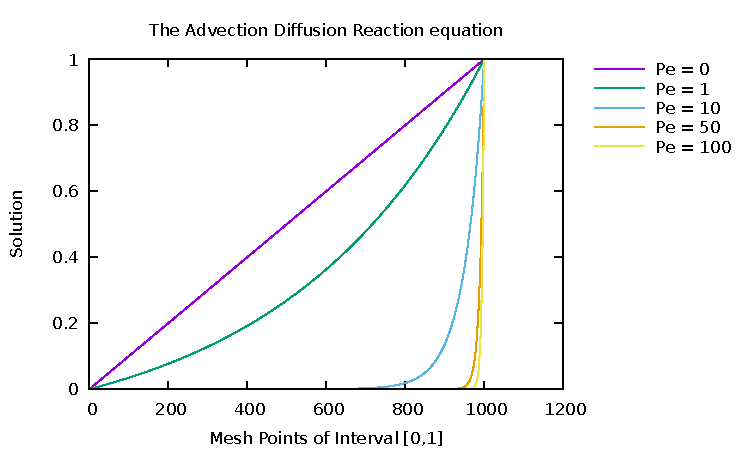
\includegraphics[width=1\textwidth]{function_1000}
  \end{center}
  \caption{Here we see the approximate solutions for mesh size h = 0.001.
  \label{fig:func_and_deriv}}
\end{figure}

 \begin{figure}
 \begin{center}
    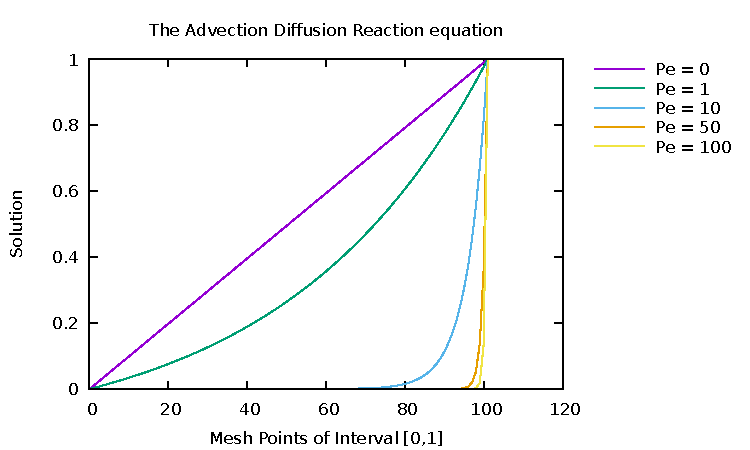
\includegraphics[width=1\textwidth]{function_100}
  \end{center}
  \caption{Here we see the approximate solutions for mesh size h = 0.01.
  \label{fig:func2}}
\end{figure}

 \begin{figure}
 \begin{center}
    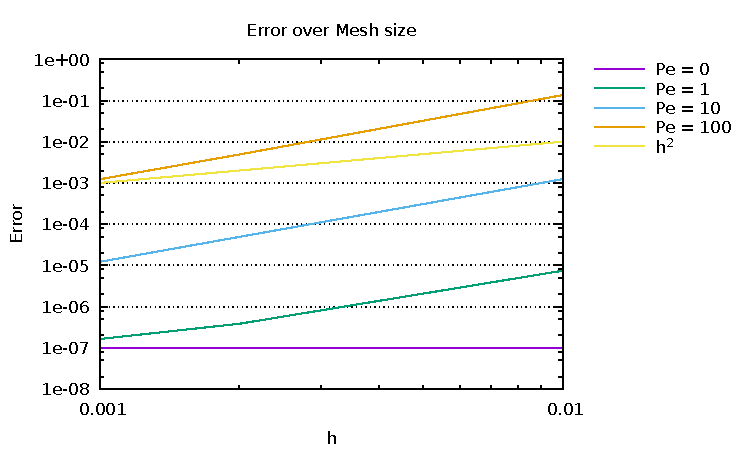
\includegraphics[width=1\textwidth]{error}
  \end{center}
  \caption{The figure shows the error incurred as the mesh size h varies. Except for Pe = 0, the order of convergence is at least 2.
  \label{fig:func2}}
\end{figure}


\end{document}
